\section{Računanje z ulomki}

\begin{frame}
    \sectionpage
\end{frame}

\begin{frame}
    \tableofcontents[currentsection, hideothersubsections]
\end{frame}

    \subsection{Ulomki z enakimi imenovalci}

        \begin{frame}[t]
            \frametitle{Ulomki z enakimi imenovalci}

            \begin{alertblock}{}
                Ulomke z enakimi imenovalci \textbf{seštevamo} tako, da \textbf{seštejemo števce}, \textbf{imenovalce} pa \textbf{prepišemo}.
                $$ \mathbf{\frac{a}{c}+\frac{b}{c}=\frac{a+b}{c}}, $$ pri pogoju, da $c\neq 0$.

                Ulomke z enakimi imenovalci \textbf{odštevamo} tako, da \textbf{imenovalec prepišemo}, števec pa izračunamo tako, da \textbf{od števca prvega ulomka odštejemo števec drugega ulomka}.
                $$ \mathbf{\frac{a}{c}-\frac{b}{c}=\frac{a-b}{c}}, $$ pri pogoju, da $a\leq b$ in $c\neq 0$.
            \end{alertblock}
        \end{frame}

    \subsection{Seštevanje ulomkov}

        \begin{frame}[t]
            \frametitle{Seštevanje ulomkov}

            \begin{alertblock}{Seštevanje ulomkov z različnimi imenovalci}
                Ulomke z \textbf{različnimi imenovalci seštevamo} tako, da jih najprej \textbf{razširimo na skupni imenovalec}, imenovalec prepišemo, števce pa seštejemo.
            \end{alertblock}

            \begin{block}{POMNI}
                Dobljeni rezultat zapišemo s celim delom in delom, manjšim od $1$.
            \end{block}

            \begin{block}{POMNI}
                Rezultat vedno zapišemo kot okrajšan ulomek.
            \end{block}

        \end{frame}

    \subsection{Odštevanje ulomkov}

        \begin{frame}[t]
            \frametitle{Odštevanje ulomkov}

            \begin{alertblock}{Odštevanje ulomkov z različnimi imenovalci}
                Ulomke z \textbf{različnimi imenovalci odštevamo} tako, da jih najprej \textbf{razširimo na skupni imenovalec}, imenovalec prepišemo, od števca zmanjševanca (prvega ulomka) pa odštejemo števec odštevanca (drugega ulomka). 
            \end{alertblock}

            \begin{block}{POMNI}
                Če moramo zaporedoma odšteti več odštevancev, odštevance seštejemo in nato odštejemo njihovo vsoto.
            \end{block}

        \end{frame}

    \subsection{Množenje ulomka z naravnim številom}

        \begin{frame}[t]
            \frametitle{Množenje ulomka z naravnim številom}

            \begin{alertblock}{}
                Ulomek \textbf{množimo z naravnim številom} tako, da \textbf{števec pomnožimo z naravnim številom}, \textbf{imenovalec} pa \textbf{prepišemo}.
                $$ \mathbf{n\cdot\frac{a}{b}=\frac{n\cdot a}{b}}, $$ pri pogoju, da $b\neq 0$.
            \end{alertblock}        
            
            \begin{exampleblock}{POZOR}
                $$ n\cdot\frac{a}{b}\neq n\frac{a}{b} $$
            \end{exampleblock}
        \end{frame}


    \subsection{Množenje ulomka z ulomkom}

        \begin{frame}[t]
            \frametitle{Množenje ulomka z ulomkom}

            \begin{alertblock}{}
                Ulomek \textbf{množimo} z ulomkom tako, da \textbf{pomnožimo števec s števcem} in \textbf{imenovalec z imenovalcem}.
                $$ \mathbf{\frac{a}{b}\cdot\frac{c}{d}=\frac{a\cdot c}{b\cdot d}}, $$ pri pogoju, da $b\neq 0, d\neq 0$.
            \end{alertblock}

            \begin{exampleblock}{POZOR}
                $$ m\frac{a}{b}\cdot n\frac{c}{d}\neq m\cdot n\frac{a\cdot c}{b\cdot d} $$
            \end{exampleblock}

            \begin{block}{POMNI}
                Rezultat naj bo vedno okrajšani ulomek. Če je mogoče, naj bo zapisan s celim delom  in ulomkom, manjšim od $1$.
            \end{block}

        \end{frame}

    \subsection{Deljenje ulomka z naravnim številom}

        \begin{frame}[t]
            \frametitle{Deljenje ulomka z naravnim številom}

            \begin{alertblock}{}
                \textbf{Ulomek delimo z naravnim številom} na dva načina:
                \begin{enumerate}
                    \item \textbf{števec} ulomka \textbf{delimo} z naravnim številom: $$\mathbf{\frac{a}{b}:n=\frac{a:n}{b}};$$
                    \item \textbf{imenovalec} ulomka \textbf{pomnožimo} z naravnim številom: $$\mathbf{\frac{a}{b}:n=\frac{a}{b\cdot n}}.$$
                \end{enumerate}
            \end{alertblock}                
            
            \begin{exampleblock}{POZOR}
                Drugi način je vedno mogoč, prvi pa le, če je števec ulomka deljiv z danim naravnim številom.
            \end{exampleblock}
        \end{frame}

    \subsection{Deljenje ulomka z ulomkom}

        \begin{frame}[t]
            \frametitle{Deljenje ulomka z ulomkom}

            \begin{alertblock}{Obratni ulomek}
                Obratna ulomka sta ulomka, katerih produkt je enak $1$.
                $$ \mathbf{\frac{a}{b}\cdot\frac{b}{a}=1} $$
            \end{alertblock}

            \begin{alertblock}{Deljenje ulomkov}
                Ulomek delimo z drugim ulomkom tako, da ga pomnožimo z obratno vrednostjo drugega ulomka.
                $$ \mathbf{\frac{a}{b}:\frac{c}{d}=\frac{a}{b}\cdot\frac{d}{c}=\frac{a\cdot d}{b\cdot c}} $$
            \end{alertblock}       

        \end{frame}



    \subsection{Številski izrazi}

        \begin{frame}[t]
            \frametitle{Številski izrazi}

            \begin{alertblock}{Vrstni red operacij}
                Pri številskih izrazih z  oklepaji \textbf{izračunamo najprej računske operacije v oklepaju}. Vedno najprej v najbolj notranjem oklepaju.

                Pri številskih izrazih brez oklepajev upoštevamo običajni vrstni red, po katerem \textbf{množimo in delimo pred seštevanjem in odštevanjem}.
            \end{alertblock}
        \end{frame}

    \subsection{Naloge z besedilo}

        \begin{frame}[t]
            \frametitle{Naloge z besedilom}

            \begin{exampleblock}{DOGOVOR}
                Vsaka naloga z besedilom zahteva tudi zapisan odgovor.
            \end{exampleblock}

            \begin{block}{POMNI}
                \begin{tabular}{|l|l|}
                    \hline 
                    operacija & rezultat \\
                    \hline \hline
                    $+$ seštevanje & vsota \\
                    \hline
                    $-$ odštevanje & razlika \\
                    \hline
                    $\cdot$ množenje & produkt \\
                    \hline
                    $:$ deljenje & kvocient \\
                    \hline 
                    
                \end{tabular}
            \end{block}
        \end{frame}

    \subsection{Izrazi s spremenljivkami}
        
        % \begin{frame}[t]
        %     \frametitle{Izrazi s spremenljivkami}
        % \end{frame}

    \subsection{Enačbe in neenačbe}
        
        % \begin{frame}[t]
        %     \frametitle{Enačbe in neenačbe}

        %     \begin{alertblock}{Reševanje enačb in neenačb}
        %         Besedilne naloge, ki vsebujejo neznane količine (enačbe ali neenačbe) rešujemo tako, da najprej \textbf{določimo neznanko}, nato \textbf{sklepamo}, nakar \textbf{rešimo nalogo} s preglednico, diagramom ali enačbo, na koncu \textbf{preverimo rezultat} in \textbf{zapišemo odgovor}.
        %     \end{alertblock}
        % \end{frame}

        \begin{frame}[t]
            \frametitle{Neenačbe}

            \begin{columns}
                \column{0.53\textwidth}
                    \only<1->{\begin{alertblock}{}
                        \textbf{Neenakost} je izjava, v kateri nastopajo znaki $<$, $>$, $\leq$ ali $\geq$.
                    \end{alertblock}}
                    \only<1-2>{~ \\ ~ \\ ~ \\ ~ \\}
                    % \only<3->{\begin{alertblock}{}
                    %     \textbf{Neenakost} je izjavna oblika, v kateri nastopajo znaki $<$, $>$, $\leq$ ali $\geq$.
                    % \end{alertblock}
                    \only<3->{ $$ 12.5 - 2 > 8 $$  $$ 3 + 6 \leq 9 $$}

                \column{0.45\textwidth}
                    \onslide<2->{\begin{table}
                        \centering
                        \addtolength{\tabcolsep}{6pt}
                        \renewcommand{\arraystretch}{1.4}                
                        \begin{tabular}{||c|c||} 
                            \hhline{|t:==:t|}
                                    $\mathbf{<}$ & manjše   \\ 
                            \hline
                                    $\mathbf{>}$ & večje   \\ 
                            \hline
                                    $\mathbf{\leq}$ & manjše ali enako   \\ 
                            \hline
                                    $\mathbf{\geq}$ & večje ali enako  \\  
                            \hhline{|b:==:b|}
                        \end{tabular}
                    \end{table}}
            \end{columns}

            \onslide<4->{\begin{alertblock}{}
                \textbf{Neenačba} je neenakost, v kateri nastopa neznanka.
            \end{alertblock}}

            \onslide<5->{$$ 0.7 + x \geq 4 $$
                $$ 3\cdot x + 5 < 17.6 $$
            }

        \end{frame}

        \begin{frame}[t]
            \only<1->{\begin{alertblock}{}
                \textbf{Osnovna množica} $\mathbf{\mathcal{U}}$ je množica števil, ki jih smemo uporabiti pri reševanju neenačbe. Če osnovna množica ni posebej izbrana, je $\mathcal{U}=\mathbb{N}_0$ (naravna števila skupaj s številom $0$). 
            \end{alertblock}}

            \only<2->{\begin{alertblock}{}
                \textbf{Rešitev neenačbe} je vsako število, za katero dobimo iz izjavne oblike pravilno izjavo. Zapišemo množico rešitev, ki jo označimo z $\mathbf{\mathcal{R}}$. 
            \end{alertblock}}

            \begin{columns}
                \column{0.32\textwidth}            
                \only<3->{$$ x + 3\frac{1}{4} < 9$$
                    $$\mathcal{R}=\left\{1,2,3,4,5\right\}$$}

               \column{0.32\textwidth}          
                \only<4->{$$\mathcal{U}=\left\{2,3,4\right\} $$
                    $$ x + 3\frac{1}{4} < 9$$
                    $$\mathcal{R}=\left\{2,3,4\right\}$$}

                \column{0.32\textwidth}          
                \only<5->{$$\mathcal{U}=\left\{10,11,12,13,14,15\right\} $$
                    $$ x + 3\frac{1}{4} < 9$$
                    $$\mathcal{R}=\left\{\right\}$$}
            \end{columns}


            \only<6->{\begin{block}{}
                Množica rešitev je odvisna od osnovne množice.
                Kadar v osnovni množici ni števila, ki reši neenačbo, je množica rešitev prazna, kar zapišemo $\mathcal{R}=\emptyset$ ali $\mathcal{R}=\left\{\right\}$.
            \end{block}}
        \end{frame}

        \begin{frame}[t]
            \begin{exampleblock}{REŠEVANJE NEENAČBE S PREMISLEKOM}
                Naj bo $\mathcal{U}=\mathbb{N}_0$. \\
                Poiskati želimo števila, ki ustrezajo neenačbi $\mathbf{2\frac{5}{7}< x \leq 8\frac{1}{3}}$. \\ ~\\
                \only<2->{Razmislimo, katera izmed naravnih števil lahko vstavimo namesto $x$-a, da bo izjava pravilna. \\}
                \only<3->{Takšna števila so: $x\in\left\{3,4,5,6,7,8\right\}$. \\}
                \only<4->{Zapišemo še množico rešitev: $\mathbf{\mathcal{R}=\left\{3,4,5,6,7,8\right\}}$.}

            \end{exampleblock}

            \only<5->{\begin{block}{PREDSTAVITEV MNOŽICE REŠITEV NA ŠTEVILSKI PREMICI}
                Na številski premici želimo predstaviti zgornjo rešitev. \\ ~ \\ \only<5>{~\\~\\}
                \only<6->{
                    \begin{figure}
                        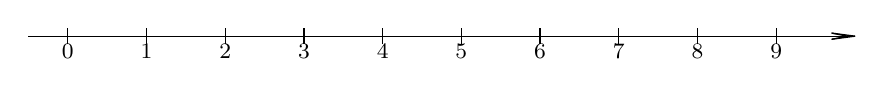
\begin{tikzpicture}
                            % \clip (0,0) rectangle (14.000000,10.000000);
                            {\footnotesize
                            
                            % Drawing segment A B
                            \draw [line width=0.016cm] (0.500000,1.500000) -- (11.000000,1.500000);%
                            
                            % Drawing arrow A B 1.00
                            \draw [line width=0.016cm] (10.702567,1.539158) -- (11.000000,1.500000);%
                            \draw [line width=0.016cm] (10.702567,1.539158) -- (10.900856,1.500000);%
                            \draw [line width=0.016cm] (10.702567,1.460842) -- (11.000000,1.500000);%
                            \draw [line width=0.016cm] (10.702567,1.460842) -- (10.900856,1.500000);%
                            
                            % Marking point 0
                            \draw (1.000000,1.500000) node [anchor=north] { $0$ };%
                            
                            % Marking point 1
                            \draw (2.000000,1.500000) node [anchor=north] { $1$ };%
                            
                            % Marking point 2
                            \draw (3.000000,1.500000) node [anchor=north] { $2$ };%
                            
                            % Marking point 3
                            \draw (4.000000,1.500000) node [anchor=north] { $3$ };%
                            
                            % Marking point 4
                            \draw (5.000000,1.500000) node [anchor=north] { $4$ };%
                            
                            % Marking point 5
                            \draw (6.000000,1.500000) node [anchor=north] { $5$ };%
                            
                            % Marking point 6
                            \draw (7.000000,1.500000) node [anchor=north] { $6$ };%
                            
                            % Marking point 7
                            \draw (8.000000,1.500000) node [anchor=north] { $7$ };%
                            
                            % Marking point 8
                            \draw (9.000000,1.500000) node [anchor=north] { $8$ };%
                            
                            % Marking point 9
                            \draw (10.000000,1.500000) node [anchor=north] { $9$ };%
                            
                            % Drawing segment 0a 0b
                            \draw [line width=0.016cm] (1.000000,1.400000) -- (1.000000,1.600000);%
                            
                            % Drawing segment 1a 1b
                            \draw [line width=0.016cm] (2.000000,1.400000) -- (2.000000,1.600000);%
                            
                            % Drawing segment 2a 2b
                            \draw [line width=0.016cm] (3.000000,1.400000) -- (3.000000,1.600000);%
                            
                            % Drawing segment 3a 3b
                            \draw [line width=0.016cm] (4.000000,1.400000) -- (4.000000,1.600000);%
                            
                            % Drawing segment 4a 4b
                            \draw [line width=0.016cm] (5.000000,1.400000) -- (5.000000,1.600000);%
                            
                            % Drawing segment 5a 5b
                            \draw [line width=0.016cm] (6.000000,1.400000) -- (6.000000,1.600000);%
                            
                            % Drawing segment 6a 6b
                            \draw [line width=0.016cm] (7.000000,1.400000) -- (7.000000,1.600000);%
                            
                            % Drawing segment 7a 7b
                            \draw [line width=0.016cm] (8.000000,1.400000) -- (8.000000,1.600000);%
                            
                            % Drawing segment 8a 8b
                            \draw [line width=0.016cm] (9.000000,1.400000) -- (9.000000,1.600000);%
                            
                            % Drawing segment 9a 9b
                            \draw [line width=0.016cm] (10.000000,1.400000) -- (10.000000,1.600000);%
                            }
                            \end{tikzpicture}
                                                        
                    \end{figure}
                }

                
            \end{block}}

        \end{frame}

        \begin{frame}[t]
            \begin{exampleblock}{REŠEVANJE NEENAČBE S PREGLEDNICO}
                Naj bo $\mathcal{U}=\left\{\frac{1}{3},\frac{2}{3},1,1\frac{1}{3}\right\}$. \\
                Rešujemo enačbo $\mathbf{x+2\frac{1}{2} < 3\frac{1}{2}}$.
                \only<2>{\begin{table}
                    \centering
                    \addtolength{\tabcolsep}{6pt}
                    \renewcommand{\arraystretch}{1.4}                
                    \begin{tabular}{|c|c|c|c|} 
                        \hline 
                                $x$ & {leva stran neenačbe: $\quad \quad \quad$} & desna stran neenačbe: $\quad$ & pravilnost    \\ 
                        \hline \hline
                                &  &  &   \\ 
                        \hline
                                 & & & \\ 
                        \hline
                                 & & & \\  
                        \hline
                                 & & & \\
                        \hline
                    \end{tabular}
                \end{table}}

                \only<3->{\begin{table}
                    \centering
                    \addtolength{\tabcolsep}{6pt}
                    \renewcommand{\arraystretch}{1.4}                
                    \begin{tabular}{|c|c|c|c|} 
                        \hline 
                                $x$ & {leva stran neenačbe: $x+2\frac{1}{2}$} & desna stran neenačbe: $3\frac{1}{2}$ & pravilnost    \\ 
                        \hline \hline
                                $\frac{1}{3}$ & $\frac{1}{3}+2\frac{1}{2}=2\frac{5}{6}$ & $3\frac{1}{2}$ &  P \\ 
                        \hline
                                $\frac{2}{3}$ & $\frac{2}{3}+2\frac{1}{2}=3\frac{1}{6}$ & $3\frac{1}{2}$ & P \\ 
                        \hline
                                 $1$ & $1+2\frac{1}{2}=3\frac{1}{2}$ & $3\frac{1}{2}$ & N \\  
                        \hline
                         $1\frac{1}{3}$ & $1\frac{1}{3}+2\frac{1}{2}=3\frac{5}{6}$ & $3\frac{1}{2}$ & N \\
                        \hline
                    \end{tabular}
                \end{table}}

                \only<4->{Zapišemo množico rešitev: $\mathbf{\mathcal{R}=\left\{\frac{1}{3},\frac{2}{3}\right\}}$.
                }
            \end{exampleblock}
        \end{frame}

        % \begin{frame}[t]
            
        %     \begin{exampleblock}{Reševanje neenačbe z ekvivalentnim preoblikovanjem}
        %         Naj bo $\mathcal{U}$ množica vseh nenegativnih števil. Rešiti želimo neenačbo $3\cdot x+4\frac{1}{2}\leq 15\frac{1}{4}$.
                
        %         \begin{columns}
        %             \column{0.45\textwidth}
        %                 \only<2->{$$3\cdot x+4\frac{1}{2}\leq 15\frac{1}{4}$$}
        %                 \only<4->{$$3\cdot x\leq 15\frac{1}{4}-4\frac{1}{2}$$}
        %                 \only<5->{$$3\cdot x\leq 10\frac{3}{4}$$}
        %                 \only<7->{$$x\leq \frac{43}{4}:3 $$}
        %                 \only<8->{$$x\leq 3\frac{7}{12}$$}
        %                 % $$x\leq 3\frac{7}{12}$$

        %             \column{0.53\textwidth}
        %                 \only<3->{Na obeh straneh neenačbe odštejemo $4\frac{1}{2}$. \\}
        %                 \only<4->{~\\}
        %                 \only<5->{~\\ ~\\}
        %                 \only<6->{Obe strani neenačbe delimo s $3$. \\}  
        %                 \only<7->{~ \\}
        %                 \only<8->{~ \\}
        %         \end{columns}
        %     \end{exampleblock}

        % \end{frame}


        % \subsection{Špela se preizkusi}
        
        % \begin{frame}[t]
        %     \frametitle{Špela se preizkusi}
        % \end{frame}